\documentclass[UTF8,11pt]{ctexart}

\usepackage[a4paper,top=22mm,bottom=24mm,left=23mm,right=23mm,headsep=7mm,footskip=12mm]{geometry}
\usepackage{microtype}
\usepackage{amsmath,amssymb,amsthm,mathtools}
\usepackage{booktabs,tabularx,array,multirow}
\usepackage{graphicx}
\usepackage{caption}
\usepackage{subcaption}
\usepackage{placeins}
\usepackage{float}
\usepackage{xcolor}
\usepackage{enumitem}
\usepackage[numbers,sort&compress]{natbib}
\usepackage[hidelinks]{hyperref}
\usepackage{fancyhdr}
\usepackage{seqsplit}

\definecolor{navy}{HTML}{17365D}
\definecolor{teal}{HTML}{00897B}
\hypersetup{colorlinks=true,breaklinks=true,linkcolor=navy,citecolor=teal,urlcolor=navy}
\graphicspath{{figures/}}
\captionsetup{font=small,labelfont=bf,labelsep=period,justification=justified,singlelinecheck=false}
\setlist{nosep,leftmargin=1.8em}
\setlength{\parskip}{0.16em}
\setlength{\parindent}{2em}
\setlength{\emergencystretch}{3em}
\setlength{\textfloatsep}{14pt plus 2pt minus 4pt}
\setlength{\floatsep}{12pt plus 2pt minus 3pt}
\setlength{\intextsep}{12pt plus 2pt minus 3pt}
\setcounter{topnumber}{4}
\setcounter{bottomnumber}{2}
\setcounter{totalnumber}{5}
\renewcommand{\topfraction}{0.90}
\renewcommand{\bottomfraction}{0.80}
\renewcommand{\textfraction}{0.08}
\renewcommand{\floatpagefraction}{0.80}
\clubpenalty=10000
\widowpenalty=10000
\displaywidowpenalty=10000
\raggedbottom
\pagestyle{fancy}
\fancyhf{}
\fancyhead[L]{面向跨域电池容量保持率估计的前缀因果损害预算投影}
\fancyhead[R]{吴雨阳、姜爱萍}
\fancyfoot[C]{\thepage}
\renewcommand{\headrulewidth}{0.4pt}
\setlength{\headheight}{14pt}

\newtheorem{lemma}{引理}
\newtheorem{theorem}{定理}
\newtheorem{corollary}{推论}
\newcommand{\R}{\mathbb{R}}

\title{\textbf{面向跨域锂离子电池容量保持率估计的\\前缀因果损害预算投影}}
\author{吴雨阳\textsuperscript{1} \quad 姜爱萍\textsuperscript{1,*}\\[0.45em]
\small\textsuperscript{1}上海大学悉尼工商学院，上海 201899\\
\small\textsuperscript{*}通讯作者：\href{mailto:ap724@shu.edu.cn}{ap724@shu.edu.cn}}
\date{}

\begin{document}
\maketitle

\begin{abstract}
车队运营方常需在参考容量测试尚不可得时，依据部分充电轨迹更新电池健康记录。跨域估计能够适应新的电池群体，但无标签部署仍缺少一种同时限制逐次更新损害并禁止未来数据改写既有估计的统一约束。本文提出前缀因果损害预算投影（prefix-causal harm-budget projection，PCHP）：将受保护源域预测与利用投运后变化的候选预测分开，再把候选投影到递归可行的非增区间。无须分布假设，PCHP 对任意隐藏结果都能把逐记录绝对损失相对于受保护状态的增量限制在声明预算内，并保持所有已发布前缀不变。在覆盖 $12$ 个开发域、$586$ 个电芯和 $601{,}932$ 条记录的嵌套评估中，PCHP 将域等权 MAE 从 $0.07524$ 降至 $0.07038$；配对差为 $-0.00486$（$95\%$ 区间 $[-0.00671,-0.00301]$），且 $11/12$ 个域改善。在六个外部数据集、$659$ 个电芯和 $9{,}712$ 条记录上的协议冻结确认中，PCHP 相对于开发数据选出的常数预算可行偏移，MAE 差为 $-0.00690$（$95\%$ 区间 $[-0.01192,-0.00212]$），并在 $5/6$ 个数据集上改善且通过全部确定性检查。结果盲的 $45$ 电芯 BaSyTec 评估进一步确认了部署约束迁移，同时揭示其精度权衡。当漏检退化的代价是不必要复核的五倍时，PCHP 将连续非对称代价降低 $7.54\%$；$0.01$ 预算未改变以 $80\%$ 容量保持率为阈值的二元复核决策。因此，PCHP 支持结果到达前的自适应跨域电池容量保持率更新，并明确控制预测损害与运维权衡。
\end{abstract}

\noindent\textbf{关键词：}锂离子电池；容量保持率；健康状态；域适配；在线预测；风险控制；电池管理

\section{引言}

设想一个正在引入新供应商电芯的换电运营商。每次服务检查时，运营方必须在“继续常规运行”和“安排完整诊断与维护复核”之间作出选择。部分充电记录已经到达，但准确参考容量仍不可得，因为受控容量表征会中断正常服务。传统估计通常依赖专门设计的充放电工况，而近期方法使用随机或部分充电片段，正是因为完整轨迹很少符合实际运行条件 \citep{liu2023rapid,zhang2024flexible}。源域模型可以立即给出容量保持率，另一模型则利用电芯相对于投运初期的充电响应变化提出更新；然而，在真实容量揭示之前，运营方无法知道该更新是否有益。这里存在明确的非对称后果：低估容量保持率会导致过早测试、停机和不必要干预，高估则可能延误对退化电芯的处理并增加运行或质保暴露。回顾性单调平滑还会产生第二类风险——下个月出现的向下异常可能改写今天已经用于决策的记录。因此，现实问题不只是提高迁移精度，而是如何在保留已发布记录的同时，在线接纳有用更新并限制其决策相关损害。

SOH 估计直接影响维护与质保决策。数据驱动模型能够利用电压、电流、充电量、温度和循环历史，而无须辨识每一条退化路径 \citep{ng2020mlbattery,roman2021pipeline}；短充电片段可用于 SOH 估计，早期寿命记录则可在完成全寿命表征之前支持寿命预测 \citep{roman2021pipeline,severson2019cyclelife}。跨域学习进一步通过表征对齐、源域选择、个性化迁移、模型集成和测试时适应降低对目标域老化标签的依赖 \citep{li2020sstca,ma2022personalized,lu2023without,duan2025wasserstein,feng2024batteryttt}。这些方法提高了异质工况下的适应能力；实际部署还需要一条清晰规则，在隐藏结果到达前限制未经验证的更新能够偏离受保护记录多远，并把过早干预与延迟干预的不等后果转化为可审计预算。

本文通过分离“效用产生”“因果状态构造”与“损害控制”来填补这一能力缺口。受保护模型使用原始早期充电特征，学习候选进一步使用相对于前五次表征记录的原量纲变化。受保护原始预测被转换为忽略向上创新、按比例 $\alpha$ 吸收向下创新的前缀因果非增状态；随后，PCHP 将当前候选投影到该状态周围的递归可行区间。整个过程不使用目标结果，不修改已经发布的前缀，并限制相对于受保护状态的最坏绝对损失增量。图~\ref{fig:workflow_zh} 概括了现实问题、方法与证据链。

\begin{figure}[t]
  \centering
  
\includegraphics[width=\textwidth]{fig1_method_workflow_zh.pdf}
  \caption{现实问题、前缀因果方法与核心证据。\textbf{A}，在线容量保持记录在未来充电数据到达后不得改变。\textbf{B}，受保护原始预测被转换为单向因果非增状态，利用投运初期变化的模型提出候选更新。\textbf{C}，PCHP 将候选投影到损害预算区间与递归可行非增集合的交集。\textbf{D}，嵌套开发评估、匹配常数偏移对照，以及结果盲、协议锁定外部验证的配对效应；区间按所述独立单位重采样。}
  \label{fig:workflow_zh}
\end{figure}

本文的核心贡献是一个输出空间算子，使学习得到的跨域更新能够在结果未知时按照明确的风险约束执行。损害预算区间是满足所声明逐记录绝对损失界的必要充分集合；它与轨迹约束的交集构成精确的递归可行集。PCHP 在其中选择最接近学习候选的输出，从而同时获得前缀不变性、非增健康记录、每次更新 $O(1)$ 的执行复杂度，以及紧的前缀 $\ell_\infty$ 非扩张保证。

证据链同时检验效用与所提出的运行机制。十二域嵌套评估衡量跨域性能；匹配常数偏移和无保护比较器分别识别记录级候选信息与保护带来的精度代价；六数据集协议冻结分析在 $659$ 个外部电芯上检验同一机制；非对称代价重放把预测误差连接到维护后果；结果盲 BaSyTec 评估检验部署约束能否迁移到新的实验项目。上述结果共同支持将 PCHP 用作自适应电池健康估计的在线损害控制层。

\section{相关工作与方法差异}

\subsection{跨域电池健康状态估计}

电池 SOH 估计已经从人工健康指标和浅层回归器发展至序列模型、物理信息学习和跨域迁移 \citep{ng2020mlbattery,roman2021pipeline,wang2024pinn}。半监督迁移成分分析通过对齐源域与目标域表征来缓解有限标签问题 \citep{li2020sstca}；深度迁移学习面向未见放电协议开展个性化健康预测 \citep{ma2022personalized}；域适配模型集成则在不新增目标域退化实验的条件下估计 SOH \citep{lu2023without}。近期研究还使用 Wasserstein 距离选择源域后再微调时序模型 \citep{duan2025wasserstein}，或利用逐步到达的无标签目标输入执行测试时训练 \citep{feng2024batteryttt}。Applied Energy 的同期研究把源域选择与保持老化顺序的对齐结合用于多源域适配 \citep{qiu2024multisource}，或通过贝叶斯混合效应迁移，根据每个电池可获得的运行信息选择参数更新方式 \citep{zhang2025bayesian}。另一项 Energy and AI 现场研究在 $3{,}000$ 辆车上结合多视图协同训练与置信度驱动的伪标签，并在标签逐步出现后将其增量纳入训练 \citep{hadzalic2025field}。这些工作表明，目标历史、概率信息共享或逐步标签能够缓解异质性。本文的问题发生在更早的信息阶段：任何目标结果尚不可得时，能否允许学习更新，同时对每个隐藏结果限制其相对损害，并禁止未来观测改写已发布记录？

同期工作进一步探索使用少量目标监督的域对抗电芯到电池包迁移 \citep{shu2026celltopack}、稀疏目标标签下的概率迁移 \citep{shao2026probabilistic}，以及结合全局单调惩罚的物理引导专家路由 \citep{jiang2026phasemoe}。面向可靠性的扩展还将域对齐与共形预测区间结合 \citep{filgueira2026conformalized}，或根据带标签现场留出集上的误差选择单调后校准器 \citep{nyachionjeka2026safecalibrated}。这些方法改进了适应能力、不确定性量化或物理一致性，但并未给出本文研究的保证。本文的目标域既不提供结果标签，也不参与参数更新：两个源域模型在目标预测前已经冻结，目标阶段只约束其输出轨迹，保证对象是逐点损失增量，而不是区间覆盖率、目标监督改善或训练惩罚。

相邻的预测与健康管理研究使上述区别更加明确。复合域偏移预测同时对齐机械退化轨迹的域间分布和域内退化阶段分布 \citep{ding2023compound}；源域开放集域泛化在训练阶段无目标域数据的条件下，面向未知工况学习故障分类器 \citep{song2026regroupment}；交互式电池预测则递归耦合神经网络容量估计与切换状态空间过程以更新剩余使用寿命 \citep{duan2025interactive}。这些工作的报告目标分别是降低表征偏移、执行仅用源域的开放集分类以及递归寿命预测。PCHP 针对不同的保证对象：在学习预测器保持冻结的条件下，围绕受保护的前缀因果状态约束与结果无关的逐记录损害预算。

BatteryML 和 BatteryLife 对异构公开老化数据进行了标准化整理，从而使大范围跨数据集评估更易复现 \citep{zhang2024batteryml,tan2025batterylife}。但数据广度也要求正确界定统计重复：循环嵌套于电芯，电芯又嵌套于完整数据集。本文因此将完整电池数据域而非单个循环作为开发阶段跨域效应的独立单位。

\subsection{负迁移与安全回归}

负迁移指迁移数据或知识降低目标性能的情形，既有缓解路线包括域相似性估计、安全迁移和显式负迁移抑制 \citep{zhang2023negative}。在安全半监督回归中，SAFER 将监督预测几何投影至多个半监督回归器构成的凸集，并在完整真实标签向量位于该集合时获得平方损失不劣结论 \citep{li2017safer}。SAFEW 将极大极小安全弱监督扩展至多种分类与回归凸损失，其保证依赖于真实标签与基学习器集合之间满足文中规定的安全条件 \citep{li2021safeweak}。专家评价者建议允许不同专家及不同时刻采用不同的适当可混合损失，但其结论是在结果到达后成立的累积遗憾界 \citep{chernov2009evaluators}；在线概率再校准同样追求校准性以及相对于基线预测器渐近消失或较低的累积遗憾 \citep{marx2025calibrated,deshpande2025calibrated}。共形校准器给出概率校准保证，并分析一种“不伤害”效率：当基础预测系统已经理想时，共形化不应使其预测分布显著变差 \citep{vovk2020conformal}。加权共形迁移利用无标签目标协变量，在协变量偏移模型下恢复边际覆盖率 \citep{tuwani2023transport}；电池领域的共形迁移则把表征对齐与校准预测区间结合 \citep{filgueira2026conformalized}。受保护在线熵匹配通过检测分类熵偏移并更新模型参数，使其在无分布偏移时经验上保持准确率与校准 \citep{bar2024protected}。带标签的电池现场数据也被用于仅在留出误差改善时选择单调后校准器 \citep{nyachionjeka2026safecalibrated}。这些都是实质性的保护机制，但其保护对象分别是条件式向量风险、累积遗憾、预测分布效率、边际覆盖率、经验留出误差或自适应训练过程，而不是任意隐藏真实值下每条已发布点预测的损失。

本文的区别在于保证对象和执行约束。其目标不是要求最终预测普遍更准，而是在不要求真实值位于候选集合的条件下，对每一个实数真实值、每一条已发布记录给出绝对损失最大增量的精确上界。该保证在真实值被观察之前即可核验，两个预测器均保持冻结，而且同一投影必须保持此前已经发布的全部非增前缀。表~\ref{tab:novelty_audit_zh} 直接比较这些信息边界与保证边界。

\begin{table}[H]
  \centering
  \caption{按照保证对象与信息边界比较相近方法。“条件”仅记录相应文献陈述保护结论时的主要条件，不评价方法优劣。}
  \label{tab:novelty_audit_zh}
  \footnotesize
  \renewcommand{\arraystretch}{0.96}
  \begin{tabularx}{\textwidth}{@{}>{\raggedright\arraybackslash}p{0.17\textwidth}>{\raggedright\arraybackslash}p{0.20\textwidth}>{\raggedright\arraybackslash}p{0.25\textwidth}>{\raggedright\arraybackslash}X@{}}
    \toprule
    方法 & 保护对象 & 信息或成立条件 & 与 PCHP 的区别 \\
    \midrule
    SAFER / SAFEW \citep{li2017safer,li2021safeweak} & 相对监督基线的完整向量损失 & 分别满足真实标签与基学习器的相应适用条件 & 离线向量或极大极小预测；没有逐记录结果一致预算或轨迹递归 \\
    专家建议 / 在线再校准 / 保守在线凸优化 \citep{chernov2009evaluators,marx2025calibrated,deshpande2025calibrated,bernasconi2021conservative} & 校准性、累积遗憾或相对默认策略的累积损失 & 结果依次到达；保守在线凸优化使用已实现损失预算 & 累积保证，而非同一记录上对所有可能结果成立的损害域 \\
    共形校准 / 迁移 \citep{vovk2020conformal,tuwani2023transport,filgueira2026conformalized} & 校准性、理想系统效率或预测集合边际覆盖率 & IID 理想基线分析或所声明的协变量偏移假设 & 保护预测分布或集合；没有相对任意基线的逐点损失预算和不可回写轨迹 \\
    受保护适应 \citep{bar2024protected} & 无偏移数据流中的准确率与校准 & 目标熵数据流更新模型参数 & 围绕训练过程的经验保持，而非冻结模型的确定性逐点证书 \\
    电池安全校准 \citep{nyachionjeka2026safecalibrated} & 目标留出误差与单调尺度 & 带标签目标留出集选择校准器 & 目标监督后校准；没有结果未知条件下的逐点证书 \\
    相对基线 / 受约束在线决策 \citep{moradipari2020stagewise,deb2025conservative,sridharan2025unknown,vaskov2024donoharm} & 累积策略损失、即时期望奖励或动作可行性 & 动作或约束反馈、探索、约束学习或反事实评估 & 保护策略或约束模型下的决策，而非对所有结果成立的逐点预测损失或已发布前缀 \\
    预测安全过滤器 \citep{wabersich2021predictive} & 动态状态与控制输入约束 & 被控对象模型、不确定性集合、备份策略与终端安全集 & 最小修改控制动作；没有隐藏结果相对损失域或不可回写预测记录 \\
    单调游走 / 移动时域滤波 \citep{samar2004moving,gorinevsky2008efficient} & 潜在单调退化趋势与滤波稳定性 & 单向过程模型或移动窗口约束优化 & 没有冻结双预测器的结果一致损害预算，也不保证已发布前缀不可回写 \\
    PCHP（本文） & 相对受保护因果状态的逐记录绝对损失增量 & 不要求目标标签、结果分布或独立性 & 精确损害预算区间与前缀因果、递归非增可行性联合成立 \\
    \bottomrule
  \end{tabularx}
\end{table}

表~\ref{tab:novelty_audit_zh} 中最接近的概念邻居是保守在线优化与相对基线的序贯决策方法。Conservative Projection 将在线凸优化器的提议投影到以默认参数为中心的保守球中，使每一轮的累积已实现损失保持在乘性容许范围内 \citep{bernasconi2021conservative}。PCHP 保护的是当前预测相对于尚未揭示结局的逐点损失，并且要求对该结局的每一个可能取值均成立，因而不能借用先前记录积累的盈余。逐阶段保守线性赌博机为相对基线动作的即时期望奖励设置下界 \citep{moradipari2020stagewise}；未知约束在线学习则把在线学习预言机的提议映射为以高概率满足已学习约束的动作 \citep{sridharan2025unknown}。保守上下文赌博机保护相对基线的累积策略损失 \citep{deb2025conservative}，反事实“不伤害”控制限制相对备选安全策略的约束违反 \citep{vaskov2024donoharm}。这些方法都提供重要的逐轮或任意时刻保护，但对象是动作、期望奖励、已学习约束或累积反馈；它们不提供针对已发布点预测的结果一致相对损失域，也不约束后续记录不得回写已发布预测前缀。

预测安全过滤器在算法结构上更为接近：它们对学习控制器提出的动作作最小修改，并通过模型预测备份策略维持状态与输入约束 \citep{wabersich2021predictive}。PCHP 同样过滤学习提议，但其可接纳对象是已发布预测而非控制动作，不确定性来自隐藏结果而非被控对象扰动；其可行核由相对损失与记录次序约束闭式给出，不需要被控对象模型、滚动预测或终端安全集。

本文的方法贡献是面向电池在线执行的一组完整组合：仅由源域学习的候选、前缀因果受保护状态、递归可行非增输出，以及精确的逐点绝对损失预算区间。标量裁剪、几何投影和负迁移本身均为既有要素或现象；本次检索未发现具有上述完整执行约束的相同方法。该结论界定的是可核验的方法区别，而非脱离检索范围的普适优先权。

损失几何扩展给出平方损失关于结果范围的精确可行性分界，并将其接入同一前缀因果递归约束。度量恒等式来自既有的度量性质，本文的增量在于运行约束集成，而不是另造度量原语。安全弱监督方法在真值集合条件下保护向量损失，而专家建议与在线再校准在结果到达后保护累积损失。

递归可行性是约束控制中的既有概念，其强形式要求对每一条可行输入序列而非仅对优化器选中的序列均保持后续可行 \citep{lofberg2012oops}。预测控制与在线优化也已经研究时变约束和依赖历史的可行集合 \citep{li2021information,garber2024projectionfree,knaup2026recursively}。这些工作的对象是动态状态、累计约束违反、动态遗憾或机会约束。PCHP 将这一原则专门化到结果尚不可见的逐点预测，并推导出一维损害预算递归所诱导的精确条件。

\subsection{单调退化趋势}

长期容量衰减支持对非增趋势施加结构约束，但实测容量也可能由于静置恢复等因素出现局部回升和波动 \citep{ma2021regeneration}。移动时域单调趋势滤波在有限活动窗口上求解约束二次规划 \mbox{\citep{samar2004moving}}；单调游走滤波进一步给出概率化移动时域模型，并分析有界输入—有界输出稳定性与非线性脉冲响应的衰减 \citep{gorinevsky2008efficient}。这些工作是与稳定性最接近的先例，但新观测到达后活动窗口可以被重新计算，其保护对象是潜在统计趋势。在线等距回归则逐次输出预测，并以事后最优单调函数为比较对象分析在线遗憾，还可扩展至平方损失之外 \citep{kotlowski2016online}；其目标是对抗式在线遗憾，而不是围绕电池特定基线提供损害保护。PCHP 在此基础上增加了完整冻结双预测器级联的增量式前缀非扩张性，并把移动损害预算区间与不可回写输出前缀联合起来。电池文献也常将基于短充电或放电片段的即时推断称为“在线 SOH 估计” \citep{liu2020online}，但特征在线可用并不自动保证后续轨迹平滑器不会修改历史输出。PCHP 处理的是这一运行边界。其非增状态用于估计潜在长期趋势，可能抑制真实的短时容量恢复，因此原始测量与受保护趋势均应被保留并可审计。

\section{问题定义}

设 $i$ 表示物理电芯，$t$ 表示其有序表征记录。经验目标定义为投运归一化放电容量保持率
\begin{equation}
  y_{it}=\frac{Q_{it}}{\operatorname{median}(Q_{i1},\ldots,Q_{i5})},
  \label{eq:soh_zh}
\end{equation}
其中，前五次有效表征容量的中位数构成电芯特定的结果参照。只有在相互比较的放电容量由足够可比的协议测得时，该量才可解释为容量型 SOH 代理；否则，它描述的是特定工况下的表观容量保持率。在 $586$ 个开发电芯中，有 $58$ 个使用重复的部分荷电状态放电窗口，而不是统一的全容量表征：$48$ 个 RWTH 电芯和 $4$ 个 SNL 电芯使用 $20\%$--$80\%$ 窗口，$6$ 个 MICH\_EXP 电芯使用 $50\%$--$100\%$ 窗口。这些记录可以支持协议内归一化容量保持分析，但不能使式~\eqref{eq:soh_zh} 成为不依赖化学体系和测试协议的普适物理 SOH 定义。在预测阶段，$Q_{it}$ 与 $y_{it}$ 均不可用。预测从前五次充电记录之后开始；这些记录的充电测量而非放电容量同时构成投运特征参照。一个数据域对应同一实验来源、仪器体系、化学体系或协议所生成的一组电芯。在每个开发折中，完整目标域均排除于模型拟合和超参数选择之外。

令 $\mathcal F_{it}$ 表示记录 $t$ 时可用的信息，包括冻结的源域模型、电芯前五次充电参照，以及截至该记录已经观测到的全部充电测量。若某个在线预测仅依赖 $\mathcal F_{it}$，且在 $t$ 之后追加任意记录都不会改变已经发布的前缀，则称其具有前缀因果性。这里的“因果”采用信号处理中的信息约束含义，仅表示不访问未来记录；它不意味着学习特征识别了电化学因果效应。记 $r_{it}$ 为受保护模型的原始预测，$c_{it}$ 为学习候选，两者均只依赖 $\mathcal F_{it}$。最终输出 $p_{it}$ 需要同时满足四项要求：前缀因果、轨迹非增、声明的数值输出范围 $\mathcal Y=[0,1.3]$，以及相对于受保护因果状态 $b_{it}$ 的绝对损失预算 $\delta$。该范围是用于估计和递归计算的模型输出约束，不是经过认证的电化学有效区间或安全区间。

受保护状态是参照基线，而不是最优性断言。它的准确性决定 PCHP 在预算约束下可以调整的范围；下述定理不能把失准基线或协议不兼容的标签转化为准确估计。

\section{方法}

\subsection{早期充电特征与相对投运初期的变化}

每条表征记录由充电开始后的前 $600\,\mathrm{s}$ 数据构造。该窗口是固定的经过时间窗口，而不是相同的荷电状态窗口；不同电芯可能具有不同的起始荷电状态，并在不同电流下跨越不同的荷电状态范围。$24$ 个原始通道包括归一化累计充电量、电压均值与标准差、电压斜率、电流统计量、温度可用性与温度统计量、每隔 $60\,\mathrm{s}$ 的电压，以及 $0$、$300$ 和 $600\,\mathrm{s}$ 时的电流；模型另使用对数变换后的循环序号。缺失值以源训练折中的中位数填补，并由填补器附加缺失指示变量。因此，跨域评估检验的是对已观测协议异质性的稳健性，并不意味着不同数据集中的固定时间窗口在物理上等价。

对于第 $j$ 个原始通道，电芯 $i$ 的投运参照为
\begin{equation}
  a_{ij}=\operatorname{median}_{1\leq s\leq5}x_{ijs},
\end{equation}
原量纲有符号变化特征定义为
\begin{equation}
  d_{ijt}=x_{ijt}-a_{ij}.
  \label{eq:change_zh}
\end{equation}
受保护模型仅接收原始特征和循环序号；候选模型接收相同输入及全部 $d_{ijt}$。开发阶段曾评估归一化相对变化，但其域等权误差更高，且在参照量接近零时会放大分母噪声，因此在外部数据访问之前予以删除。该结论被明确报告为开发消融，而非独立外部发现。

两个主预测器均采用 ExtraTrees 回归，包含 $80$ 棵树，最小叶节点样本数为 $20$，特征子采样比例为 $0.8$，随机种子固定为 $20{,}260{,}801$。每个源域物理电芯最多保留 $80$ 个沿时间均匀抽取的记录。受保护基线采用普通合并样本权重；候选模型则使每个源数据域具有相同的总权重，避免大型档案仅因循环数量更多而主导模型。目标域推理过程中不使用结果标签，不进行微调或源域选择。

为明确候选模型各组成部分的贡献，事后开发审计采用 $2\times2$ 因子设计，交叉比较原始特征与投运参照变化特征，以及合并样本权重与域等权。四个实验臂使用完全相同的留一域外验证划分，以原始特征加合并权重模型作为受保护预测器，复用冻结的逐外层域 $\alpha$ 日程，并以完整留出数据域作为独立分析单位。最终选用的变化特征加域等权实验臂对权威预测账本实现了精确复现。

主分析完成后，本文在保持 PCHP 约束不变的条件下，分别替换三个未额外调参的表格骨干和一个轻量电池序列 Transformer，以审计架构可移植性；完整模型规格和结果移入补充材料。


\subsection{前缀因果受保护状态与损害预算投影}

记 \(\Pi_{\mathcal Y}\) 为到 \(\mathcal Y\) 的标量截断。对单个物理电芯，PCHP 按下式更新受保护状态：
\begin{align}
  b_{i1}&=\Pi_{\mathcal Y}(r_{i1}),\\
  b_{it}&=\Pi_{\mathcal Y}\!\left[b_{i,t-1}
  +\alpha\min\{r_{it}-b_{i,t-1},0\}\right],\qquad t>1,
  \label{eq:causal_state_zh}
\end{align}
其中 \(\alpha\in(0,1]\) 仅使用源域选择。该递推忽略向上创新，并按比例 \(\alpha\) 同化向下创新，因此 \(b_{it}\leq b_{i,t-1}\)。每个状态只依赖上一状态和当前原始预测，未来记录到达后不会改写已经发布的前缀。

令 \(p_{i0}=1.3\)。在记录 \(t\)，可行区间与发布输出分别为
\begin{align}
 I_{it}
 &=\left[\max\{0,b_{it}-\delta\},
 \min\{1.3,b_{it}+\delta,p_{i,t-1}\}\right],
 \label{eq:feasible_interval_zh}\\
 p_{it}&=\Pi_{I_{it}}(c_{it}).
 \label{eq:method_zh}
\end{align}
上一条发布输出保证轨迹不可回写且非增，\(b_{it}\) 周围的区间则限制学习候选能够引起的位移。

\begin{theorem}[可执行的轨迹约束]
\label{thm:pchp_zh}
若 \(b_{it}\) 遵循式~\eqref{eq:causal_state_zh} 且 \(\delta\geq0\) 为常数，则对每条记录，\(I_{it}\) 均非空。式~\eqref{eq:method_zh} 具有前缀因果性，取值属于 \(\mathcal Y\)，随记录序号非增，并满足 \(|p_{it}-b_{it}|\leq\delta\)。
\end{theorem}

\begin{theorem}[前缀层面的非扩张性]
\label{thm:nonexpansive_zh}
考虑具有相同 \(\alpha,\delta,\mathcal Y\) 和初始化、但输入流分别为 \((r,c)\) 与 \((\widetilde r,\widetilde c)\) 的两次运行。对任意截止到 \(t\) 的前缀，其输出满足
\begin{equation}
 \max_{1\leq s\leq t}|p_{is}-\widetilde p_{is}|
 \leq
 \max\!\left\{
 \max_{1\leq s\leq t}|r_{is}-\widetilde r_{is}|,
 \max_{1\leq s\leq t}|c_{is}-\widetilde c_{is}|
 \right\}.
 \label{eq:prefix_nonexpansive_zh}
\end{equation}
Lipschitz 常数 \(1\) 是紧的。
\end{theorem}

\subsection{结果一致损害的精确几何}

对损失函数 \(\ell\)、结果集合 \(\mathcal Z\)、受保护预测 \(b\) 和预算 \(\delta\)，定义
\begin{equation}
 \mathcal H^\ell_\delta(b;\mathcal Z)
 =\left\{p:\sup_{y\in\mathcal Z}
 [\ell(p,y)-\ell(b,y)]\leq\delta\right\}.
 \label{eq:generic_harm_region_zh}
\end{equation}

\begin{theorem}[绝对损失的精确可行域与零预算边界]
\label{thm:harm_region_zh}
对任意 \(b,p\in\mathbb R\)，均有
\begin{equation}
 \sup_{y\in\mathbb R}\bigl(|p-y|-|b-y|\bigr)=|p-b|.
 \label{eq:harm_region_zh}
\end{equation}
因此 \(\mathcal H^{|\cdot|}_\delta(b;\mathbb R)=[b-\delta,b+\delta]\)，且
\begin{equation}
 I_{it}=\mathcal H^{|\cdot|}_\delta(b_{it};\mathbb R)
 \cap\mathcal Y\cap(-\infty,p_{i,t-1}]
 \label{eq:maximal_interval_zh}
\end{equation}
是同时满足取值范围、已发布前缀次序与结果一致绝对损失预算的最大当前输出集合。当 \(\delta=0\) 时，只有 \(p=b\) 可行。
\end{theorem}

\begin{corollary}[精确可延拓域与最接近候选的更新]
\label{cor:viability_kernel_zh}
\label{cor:optimality_zh}
对受保护状态任意有限的未来非增延拓，每个 \(q\in I_{it}\) 均存在满足约束的输出延拓；每个 \(q\notin I_{it}\) 则已经违反当前约束。因此，\(I_{it}\) 是精确的在线可延拓域，而 \(p_{it}=\Pi_{I_{it}}(c_{it})\) 是其中唯一最接近学习候选的点。
\end{corollary}

结合定理~\ref{thm:pchp_zh} 与定理~\ref{thm:harm_region_zh}，对每条记录尚未观测的真实结果均有
\begin{equation}
 |p_{it}-y_{it}|-|b_{it}-y_{it}|
 \leq |p_{it}-b_{it}|\leq\delta.
 \label{eq:pointwise_harm_zh}
\end{equation}
该保证是确定性的，因此在任意非负加权聚合下仍然成立；实际效用的不确定性则是另一问题，必须遵循“数据域—电芯—记录”的层级。完整证明、受保护状态的近端表示、度量损失与有界平方损失的精确可行域、方向加权损失以及时变预算的可行条件均移入补充材料的理论附录。这些扩展说明部署约束如何随损失函数和声明的结果集合而变化；实验采用绝对损失，是因为它无需预设隐藏结果有界即可给出有限证书。

\subsection{计算结构}

两个冻结回归器生成当前记录预测后，PCHP 只需保存 $(b_{i,t-1},p_{i,t-1})$，并执行常数次标量运算。因此，模型推理之后，每条记录只需 $O(1)$ 状态与 $O(1)$ 时间。审计链记录 $r_{it}$、$c_{it}$、$b_{it}$、$I_{it}$、$p_{it}$、$\alpha$ 与 $\delta$。与回顾性等距回归不同，在线阶段无须对完整轨迹排序，也无须在未来记录到达后重新计算历史输出。

\section{实验设计}

\subsection{开发数据域与嵌套模型选择}

开发数据由 BatteryLife 处理数据快照（v11）、BatteryML、Battery Archive，以及 CALCE、HNEI、HUST、MATR、MICH、MICH\_EXP、RWTH、SNL、UL\_PUR、SDU 与 XJTU 各数据域对应的原始实验来源标准化整理 \citep{zhang2024batteryml,tan2025batterylife,batterylife2026processed,batteryarchive,xing2013ensemble,devie2018variability,ma2022personalized,severson2019cyclelife,attia2020closedloop,weng2021formation,li2021oneshot,preger2020degradation,juarezrobles2020safety,wang2025sorting,wang2024pinn}。去除前五次参照窗口后，分析语料包括 $12$ 个完整数据域、$586$ 个物理电芯和 $601{,}932$ 条记录，见表~\ref{tab:data_zh}。这 $12$ 个数据域均已在方法开发阶段打开，因此归类为内部或复用证据，而不是外部评估。

\begin{table}[H]
\centering
\caption{前五次参照窗口后的开发语料。记录嵌套于物理电芯，电芯嵌套于完整数据域。}
\label{tab:data_zh}
\begin{tabular}{lrr@{\qquad}lrr}
\toprule
数据域 & 电芯数 & 记录数 & 数据域 & 电芯数 & 记录数 \\
\midrule
CALB & 27 & 2,629 & MICH\_EXP & 18 & 6,455 \\
CALCE & 13 & 14,233 & RWTH & 48 & 105,140 \\
HNEI & 14 & 15,085 & SDU & 86 & 48,716 \\
HUST & 77 & 145,735 & SNL & 61 & 96,092 \\
MATR & 169 & 139,148 & UL\_PUR & 10 & 2,195 \\
MICH & 40 & 19,681 & XJTU & 23 & 6,823 \\
\midrule
\multicolumn{4}{r}{合计} & 586 & 601,932 \\
\bottomrule
\end{tabular}
\end{table}

这里的数据域并非单纯的文件标识：留出域在正极化学体系、石墨或含硅负极、圆柱/软包/方形形态、标称容量、温度、倍率、荷电状态区间及老化协议上均存在差异。补充材料表~S1 和表~S2 给出了开发数据与外部数据的完整工程属性清单；原始来源中不可用的字段统一标为 NR，不作推断或填补。

为使样本构建过程可以逐级核验，表~\ref{tab:sample_flow_zh} 分别报告来源电芯清单、特征参照资格、结果参照资格和最终评分集合。全部资格均由冻结的结构与最小历史长度规则决定，从不依据模型精度或效应方向筛选。开发数据的 $605{,}005$ 条候选循环记录经 $143$ 条结构性剔除后得到 $604{,}862$ 条符合数据约定的特征记录；再对 $586$ 个电芯各保留前五条投运参照记录、不纳入评分，恰好得到 $601{,}932$ 条评分记录。六个外部数据集共有 $945$ 个来源电芯，其中 $286$ 个不满足预设的特征参照要求，最终形成完整的 $659$ 电芯评分清单。三个导入报告未统一保留可比的上游原始记录总数，本文据实标为 NR，不作反推。补充材料表~S3 和表~S4 给出逐数据集账本及全部排除原因。

\begin{table}[H]
\centering
\caption{证据与样本流汇总。重复记录嵌套于物理电芯之内，不能解释为相互独立的样本量。}
\label{tab:sample_flow_zh}
\footnotesize
\setlength{\tabcolsep}{3.5pt}
\begin{tabularx}{\textwidth}{@{}>{\raggedright\arraybackslash}X*{5}{>{\centering\arraybackslash}p{1.65cm}}@{}}
\toprule
证据集合 & 来源电芯 & 特征参照合格 & 结果参照合格 & 评分电芯 & 评分记录 \\
\midrule
开发数据（12 个域） & 586 & 586 & 586 & 586 & 601,932 \\
外部确认（6 个数据集） & 945 & 659 & 659 & 659 & 9,712 \\
BaSyTec & 48 & 47 & 45 & 45 & 2,969 \\
\bottomrule
\end{tabularx}
\end{table}

外层评估每次留出一个完整目标域，两个回归器只在其余十一个数据域上拟合。在这些源域内部，对每一个候选值
\[
\alpha\in\{1,0.5,0.2,0.1,0.05,0.03,0.02,0.015,0.01,0.005\}
\]
再次逐域留出，并在其余十个数据域上拟合模型。先计算每个电芯的 MAE，再在域内对电芯等权平均并在域间等权平均；使该内层域等权 MAE 最小的 $\alpha$ 用于外层折。当差异不超过 $10^{-12}$ 时选择较大的 $\alpha$。外层目标域标签从不参与这一选择。全部因果分析均固定使用 $\delta=0.01$ 个归一化容量单位的损害预算。由于该预算形成于开发阶段，其工程决策含义必须由实际运营方给出，不能从外部压力测试中反推。

对每个电芯，首先在其全部参照窗口后记录上计算 MAE；随后在域内对电芯等权平均，最后对 $12$ 个数据域等权平均。主要开发估计量是 PCHP 与其 $\alpha$ 匹配受保护因果基线之间的域等权配对差。该层级避免大型数据档案或长寿命电芯支配跨域结论。

闭式损失扩展和完整递归算子在写入稿件之前均通过冻结、无标签验证器核验；穷举局部网格、随机轨迹协议、容差和工件哈希统一报告于补充材料。

\subsection{机制检验与区分性控制}

嵌套评分前，最小机制检验只使用不含标签的开发预测。在轨迹比例 $0.25$、$0.50$ 和 $0.75$ 处，本文比较仅用当前前缀计算的输出与完整未来轨迹到达后重新计算的相同历史位置。若变化超过 $10^{-4}$ 个归一化容量单位，则记为一次回顾性修订。因果机制必须保持最大前缀差为 $0$；完整轨迹等距回归则应在至少九个数据域中修改不少于一半电芯的历史前缀。第二项干预在单条受保护原始预测上加入 $+0.05$ 或 $-0.05$ 的创新。预期特征为：正向创新被完全拒绝，负向创新即时按 $\alpha$ 同化，并且相对于 $\alpha=1$，$\alpha=0.02$ 应在至少九个数据域中对不少于 $95\%$ 的干预降低累计扰动。

主要比较对象是使用同一源域选择 $\alpha$ 生成的因果受保护基线。回顾性等距损害预算方法仅作为信息泄漏诊断：它能够访问完整目标轨迹，因此不满足本文的在线执行信息边界。最强替代解释是，PCHP 可能只是把受保护状态在同一损害预算区间内做常数偏移。为检验该解释，匹配常数偏移对照对每个外层折仅使用十一个源域，联合选择 $\alpha$ 和 $\{-0.01,-0.009,\ldots,0.01\}$ 中的常数偏移。该对照与 PCHP 具有相同的取值范围、单调性和损害预算约束。

在开发结果已经打开之后，本文进一步协议锁定了一项回顾性预算路径敏感性分析，用于检验上述区分是否依赖于单一设定 $\delta=0.01$。计算前冻结
\[
\delta\in\{0,0.0025,0.005,0.0075,0.01,0.015,0.02,0.03\},
\]
原始 $\alpha$ 网格、外层数据域划分、唯一的积分主要估计量、bootstrap 随机种子 $20{,}260{,}811$ 以及判定标准。对每个外层数据域、预算和 $\alpha$，匹配常数偏移对照先计算源域残差的加权中位数，即使内层域等权电芯绝对误差最小的精确常数偏移，再将其截断到 $[-\delta,\delta]$；随后仍只用同一组十一个源域选择 $\alpha$。两项选择均不使用外层目标域标签。零预算组必须严格复现受保护状态，所有预算组均须通过声明的位移、遗憾、取值范围和单调性检查。该分析虽在执行前锁定协议，但仍属于回顾性分析，而非新的确认实验。

本文还构造了更强的\emph{无保护}因果比较器，用于度量损害控制带来的精度权衡。对每个外层目标域，仍采用仅用源域的双重留出设计，为下式选择 $\alpha$：
\[
q_{i1}=\Pi_{[0,1.3]}(c_{i1}),\qquad
q_{it}=\Pi_{[0,1.3]}\!\left(q_{i,t-1}+\alpha\min(c_{it}-q_{i,t-1},0)\right).
\]
该比较器具有前缀因果性、取值有界且轨迹非增，但不受保护基线周围损害预算区间的约束。十二个外层折均仅根据源域选择 $\alpha=0.05$。因此，它是运行上较强的精度参照，而不是具有相同损害控制的基线。

在全部开发结果已经打开后，本文实施回顾性轨迹合同消融，原样复用 V374 冻结账本且不重新拟合。逐点损害管道实验臂只移除上一条发布输出形成的上界，同时保留当前严格受保护状态、原始候选、$[0,1.3]$ 取值范围和 $\delta=0.01$ 损害管道；严格实验臂即当前 PCHP。有界恢复实验臂复用 V374 仅利用源域选择的合同，允许受保护状态和输出按所选逐记录额度回升。因此，逐点管道与严格 PCHP 的比较单独识别输出单调性，有界恢复则作为另一种状态—输出合同单独报告。

另一项回顾性范围审计检验数值输出上限本身是否决定结果。该审计不重新拟合或选择模型，而是在保存的投影前预测账本上，以 $1.1$、$1.2$、$1.3$ 和 $1.5$ 为上限完整重放算子。与主要任务目标兼容的证据包括十二域开发账本、六个外部数据集和 BaSyTec。每个设定均重新计算电芯级和数据域级 MAE、输出变化数、截断记录数，以及取值范围、轨迹、位移和观测损失证书；包含目标不兼容压力数据在内的完整范围审计见补充材料。

\subsection{协议冻结的外部机制确认与决策代价分析}

本文进一步在六个未影响十二域 PCHP 方法与评价方案设计的外部电池数据集上冻结机制确认协议：A123 石墨/LFP 一次与二次寿命研究、Imperial M50T 21700 研究、Luh NMC/C--SiO 老化研究、ILCC 变使用条件研究、Stanford 日历老化研究，以及多阶段 21700 老化研究 \citep{wheeler2025lfp,kirkaldy2024comprehensive,luh2024dataset,li2024varyingusage,lam2025calendar,stroebl2024multistage}。六个处理后数据清单依次包含 $20$、$40$、$180$、$244$、$30$ 和 $145$ 个电芯，共形成 $9{,}712$ 条参照后记录。这些数据档案曾在相互独立的探索分支中被打开，但其中的结果、汇总或比较均未参与 PCHP、特征、$\alpha=0.01$、$\delta=0.01$、常数偏移比较器、估计量、bootstrap 或判定标准的确定。因此，本文将该分析界定为协议冻结的外部机制确认，而非前瞻盲法采集。

两个冻结回归器仅在完整十二域开发数据上按既定 ExtraTrees 规格重新拟合一次，外部数据集标签不参与拟合或选择。匹配常数偏移对照采用开发数据精确选出的常数预算可行偏移：域—电芯等权残差的加权中位数为 $0.0119494$，经损害预算截断后固定为 $+0.01$。外部主要估计量为
\begin{equation}
\Delta_{\mathrm{ext}}=\frac{1}{6}\sum_{d=1}^{6}
\left(\operatorname{MAE}^{\mathrm{cell}}_{d,\mathrm{PCHP}}-
\operatorname{MAE}^{\mathrm{cell}}_{d,\mathrm{shift}}\right),
\label{eq:external_estimand_zh}
\end{equation}
其中先在电芯内对记录平均，再在每个数据集内对电芯等权平均。冻结判定标准要求 $\Delta_{\mathrm{ext}}<0$、至少四个数据集改善、两阶段数据集—电芯 bootstrap 区间上界小于零，并通过位移、观测遗憾、取值范围、单调性和前缀重放的全部精确检查。

为把预测连接到实际运维，定义复核动作 $a(p)=\mathbf 1\{p\leq\tau\}$。不必要复核的标准化代价为一，未复核真实退化电芯的代价为其 $r$ 倍：
\begin{equation}
C_{\tau,r}(p,y)=\mathbf 1\{y>\tau,\,p\leq\tau\}
+r\,\mathbf 1\{y\leq\tau,\,p>\tau\}.
\label{eq:binary_decision_cost_zh}
\end{equation}
鉴于硬阈值会掩盖尚未跨越动作边界的风险严重度变化，协议同时冻结连续非对称代价
\begin{equation}
L_r(p,y)=(y-p)_{+}+r(p-y)_{+}.
\label{eq:continuous_decision_cost_zh}
\end{equation}
主要设定为 $\tau=0.80$、$r=5$，并保留 $\tau\in\{0.70,0.80,0.90\}$ 与 $r\in\{1,2,5,10\}$ 的敏感性分析。$80\%$ 容量保持率是电动汽车一次寿命退役的常见约定，而不是普适安全阈值 \citep{saxena2015eol,montes2022secondlife}。仅当 PCHP 降低式~\eqref{eq:binary_decision_cost_zh} 时，才允许提出二元动作收益主张；否则按协议记录为非主张结果。

冻结分析完成后，本文又补充了观测随访区间内的运维重放：对每个电芯定义真实容量保持率与预测值首次越过阈值的记录。若预测越阈晚于真实越阈则记为迟报，早于真实越阈则记为过早复核，同一条记录越阈则记为准时；若预测在随访结束前未越阈，则把受限延迟截尾到末次观测后的第一条记录。报告指标包括受限绝对延迟、迟报延迟的第 $95$ 百分位数、电芯级迟报/过早/准时率，以及先在电芯内计算再等权汇总的假阴性和假阳性记录率。这些量只描述已观测区间，不外推未观测的寿命终点。

\subsection{结果盲、协议锁定的 BaSyTec 外部验证}

拜罗伊特退化路径数据集包含 $48$ 个标称容量为 $120\,\mathrm{mAh}$ 的 NMC/石墨商用电芯，在 $24$ 组温度—倍率组合下进行 $70$ 个老化循环，每个工况名义上有两个重复电芯 \citep{ramasubramanian2025degradation,roder2025degradationdata}。该批电芯在 $25\,^{\circ}\mathrm{C}$、$0.5C$、放电至 $3.0\,\mathrm{V}$ 的 CCCV 初始表征中容量为 $124\pm2\,\mathrm{mAh}$；标准参考性能测试同样使用 $25\,^{\circ}\mathrm{C}$ 与 $0.5C$ 充放电，而老化循环覆盖 $0$--$55\,^{\circ}\mathrm{C}$ 与 $0.5C$--$1.5C$。评分前，本文固化了 Zenodo 公开记录、全部 $48$ 个电芯压缩包及其官方校验和。第一版解析协议在读取任何容量数值之前闭门失败：原始导出只包含累计电量字段 \texttt{Ah[Ah]}，没有逐循环容量字段；该失败被完整保留。在查看任何累计电量数值之前，F0001 被永久指定为解析开发电芯并排除于确认。随后对其余 $47$ 个压缩包执行只读表头、零数据行的结构普查，在预测前冻结两类分隔符和四种表头签名。

对循环 $c$ 内相邻行 $j-1,j$，记累计电量为 $A_j$、电流为 $I_j$，冻结的循环放电容量恢复式为
\begin{equation}
Q_c=\sum_{j=2}^{n_c}\mathbf{1}\!\left(I_j<-10^{-5}\,\mathrm{A}\right)
\max(A_{j-1}-A_j,0).
\label{eq:basytec_capacity_zh}
\end{equation}
标签盲阶段只选择循环标识以及充电侧时间、电流和电压；数值小时乘以 $3600$ 转换为秒，随后提取固定 $600\,\mathrm{s}$ 充电窗口。在计算式~\eqref{eq:basytec_capacity_zh} 之前，程序为 $47$ 个电芯生成并哈希冻结 $3{,}101$ 条参照后预测。评分程序随后按式~\eqref{eq:soh_zh} 构造目标。由于 $Q_c$ 来自各老化循环的放电轨迹重建，而不是来自标准参考性能测试，该外部终点是工况特定的表观放电容量保持率，不是标准化 RPT SOH。电芯必须满足前五循环中位容量位于 $[0.08,0.16]\,\mathrm{Ah}$，并至少具有十条参照后标签。该容量区间是围绕电芯标称尺度预先声明的模型支持域与适用性筛选条件，不是物理有效区间或安全区间。PCHP 固定使用 $\alpha=0.01$、$\delta=0.01$；无保护边界使用源域选择的 $\alpha=0.05$。

判定标准要求至少 $36$ 个合格电芯、电芯等权配对 MAE 差为负、至少三分之二非并列电芯改善、电芯 bootstrap $95\%$ 区间上界小于 $0$，且最大逐点位移、最大观察绝对损失遗憾和最大电芯级 MAE 增量均不超过 $0.01$（容差 $10^{-12}$）。其余 $47$ 个电芯没有参与方法、超参数、估计目标、排除规则或判定标准开发，当前工作区还记录了容量访问前的预测哈希。因此，本文将其界定为基于留出公开数据的结果盲、协议锁定外部验证。该标签描述的是冻结后的评估顺序；数据此前已经采集并公开，所以这既不是前瞻采集的实验室研究，也不是独立实验室重复。

\subsection{统计分析}

全部不确定性计算均服从相应科学主张的层级。开发比较以 \(12\) 个完整留出域为配对单位；六数据集确认采用“数据集—电芯”两阶段 bootstrap；BaSyTec 以物理电芯为单位。除另有说明外，区间均使用固定随机种子和 \(100{,}000\) 次重采样。适用时，精确符号翻转分析穷举全部 \(2^{12}\) 个开发域或 \(2^6\) 个外部数据集符号分配。只有三个次级骨干比较构成多重校正家族，并使用 Bonferroni 调整后的 \(98.33\%\) 区间。重复记录从不计作独立重复。完整估计量、随机种子、有限样本敏感性、来源组聚合和多重性边界均报告于补充材料。

对于预先规定的预算路径分析，逐域汇总量定义为
\begin{equation}
A_d=\frac{1}{0.03}\int_{0}^{0.03}
\left[\operatorname{MAE}^{\mathrm{PCHP}}_d(\delta)-
\operatorname{MAE}^{\mathrm{shift}}_d(\delta)\right],\mathrm d\delta,
\label{eq:budget_auc_zh}
\end{equation}
该积分在冻结网格上采用梯形法计算，随后对 \(12\) 个域等权平均。

\section{结果}

针对闭式损失扩展和完整算子的全部冻结、无标签检查均已通过；公式差、边界检查、递归诊断与工件哈希统一报告于补充材料的验证记录。

\subsection{因果算子避免未来修订并呈现预期冲击响应}

预先设定的机制检验满足两项判定标准。完整轨迹等距回归在全部 $12$ 个数据域中修改了超过一半的电芯前缀，而因果前缀与其位于任意未来扩展中的同一前缀之间，最大差值严格为 $0$。施加 $+0.05$ 的受控创新后，单向受保护状态的最大扰动为 $0$；施加 $-0.05$ 创新后，在已保存干预明细表中，即时响应相对于理论值 $\alpha\times0.05$ 的最大误差不超过 $2.00\times10^{-16}$，处于浮点容差范围内。相对于 $\alpha=1$，$\alpha=0.02$ 在每个数据域中均对至少 $95\%$ 的干预降低了累计冲击扰动。图~\ref{fig:causality_zh} 表明，该机制确实改变了信息边界，而不是把离线平滑重新命名。

\begin{figure}[t]
  \centering
  
\includegraphics[width=\textwidth]{fig3_prefix_causality_zh.pdf}
  \caption{覆盖 $12$ 个开发数据域和 $586$ 个物理电芯的机制检验。\textbf{A}，未来记录追加后，历史离线输出变化超过 $10^{-4}$ 的电芯比例；PCHP 的最大前缀差为 $0$，虚线表示预先设定的半数电芯判定标准。\textbf{B}，$\alpha=1$ 与 $\alpha=0.02$ 下累计冲击扰动的逐域中位数配对，横轴采用对数尺度；每个数据域中的全部干预均得到改善。记录和干预嵌套于电芯，完整数据域是跨域评估单位。}
  \label{fig:causality_zh}
\end{figure}

回顾性约束审计支持上述机制解释。仅移除上一输出上界后，逐点实验臂在 \(483/586\) 个电芯上产生 \(38{,}580\) 次向上修订，而严格 PCHP 的向上修订数为零；严格实验臂相对于逐点实验臂的平均精度差为 \(+0.00026\)，其 \(95\%\) 区间跨越零。另一项完整重放表明，当输出上限在 \(1.1\) 至 \(1.5\) 之间变化时，开发数据、六个外部数据集和 BaSyTec 的输出均不改变，说明保留的 \(1.3\) 上限是计算边界，而非依据精度调出的常数。完整三臂消融与范围敏感性结果见补充材料。

\subsection{嵌套源域选择在损害预算内提高跨域效用}

在严格嵌套留一数据域评估中，PCHP 将域等权 MAE 从因果受保护基线的 $0.07524$ 降至 $0.07038$，相对降低 $6.46\%$。这里先计算每个电芯的 MAE，再在域内对电芯等权平均，最后在域间等权平均。配对差为 $-0.00486$；对完整数据域重采样得到的 $95\%$ 百分位 bootstrap 区间为 $[-0.00671,-0.00301]$。其中 $11$ 个数据域改善，无平局，仅一个数据域恶化。最大域层级损害为 $0.00109$，明显小于 $0.01$ 的逐记录预算。图~\ref{fig:domain_effects_zh} 展示全部数据域，避免把 $601{,}932$ 条重复记录误作独立跨域证据。

\begin{figure}[t]
  \centering
  
\includegraphics[width=0.92\textwidth]{fig2_domain_effects_zh.pdf}
  \caption{全部 $12$ 个外层目标域的 PCHP 减基线配对 MAE。每个点代表一个对电芯级 MAE 等权聚合后的完整数据域，负值表示 PCHP 更优。菱形及水平区间分别为域等权均值和对完整数据域执行 $100{,}000$ 次百分位 bootstrap 得到的 $95\%$ 区间。}
  \label{fig:domain_effects_zh}
\end{figure}

因果方法的点估计也低于回顾性损害预算方法，即 $0.07038$ 对 $0.07232$。两者配对差为 $-0.00195$，$95\%$ 区间为 $[-0.01073,0.00606]$。该比较不能证明因果版本在统计上更优；它只说明，在已打开的开发语料中，落实在线执行信息边界没有呈现明确的域层级精度代价。

$2\times2$ 归因审计表明，相对于投运参照的变化特征是候选模型效用的主要来源。投影前，在合并权重和域等权设定下，以变化特征替代原始特征分别使域等权电芯宏平均 MAE 降低 $0.02105$ 和 $0.02474$。经过 PCHP 后，相应降幅为 $0.00566$（基于完整域重采样的 $95\%$ 区间按降幅计为 $[0.00235,0.00941]$，精确符号翻转 $p=0.0078$）和 $0.00550$（$[0.00184,0.00970]$，$p=0.0103$）。相比之下，PCHP 层中域等权相对于合并权重的效应在原始特征和变化特征下分别为 $-0.00037$ 与 $-0.00021$，且区间均跨越零。因此，稳健增益主要归因于参照相对表征；域等权仍用于控制数据规模不平衡，但不被表述为已经单独证实的精度贡献。

\subsection{学习候选提供了超越常数预算可行偏移的信息}

匹配常数偏移对照的域等权 MAE 为 $0.07515$，PCHP 为 $0.07038$，相对降低 $6.35\%$。以 PCHP 减对照表示，配对差为 $-0.00477$，域 bootstrap $95\%$ 区间为 $[-0.00808,-0.00159]$。PCHP 在 $9$ 个数据域改善，在 $3$ 个数据域恶化，相对于该对照的最大域损害为 $0.00424$。

协议锁定的回顾性预算路径把控制从离散网格近似升级为精确源域最优常数偏移，并把比较扩展到零至三个归一化容量百分点。七个正预算的域等权均值均支持 PCHP；差值从 $\delta=0.0025$ 时的 $-0.00189$ 扩大至 $\delta=0.03$ 时的 $-0.01205$，且每个预算点的描述性区间均低于零。式~\eqref{eq:budget_auc_zh} 的主要预算归一化 AUC 差值为 $-0.00694$，域 bootstrap 区间为 $[-0.01108,-0.00296]$，逐域胜/平/负为 $11/0/1$。零预算恒等性以及位移、遗憾、取值范围和单调性门槛全部通过。独立哈希固定审计保留了原始验证器的失败记录，同时确认其唯一失败锚点是在 $10^{-12}$ 容差下，把高精度数值 $0.0703775121469438$ 与仅保留十位小数的 JSON 展示值比较所致；权威 CSV 汇总、全部 $12$ 个逐域数值和仅用源域的选择清单均与历史运行一致。因此，图~\ref{fig:candidate_control_zh} 削弱了“结论仅由单一预算下固定偏差修正造成”的解释，但不改变证据边界：开发结果此前已经打开，该路径属于回顾性稳健性证据，而不是独立证据。

来源组敏感性分析不依赖于把 MICH 与 MICH\_EXP 视为两个独立实验项目。合并二者后，开发主效应的来源组等权配对差为 $-0.00469$，$95\%$ bootstrap 区间为 $[-0.00667,-0.00274]$，胜/平/负为 $10/0/1$；候选控制配对差为 $-0.00467$，区间为 $[-0.00825,-0.00125]$，胜/平/负为 $8/0/3$。对主效应和候选控制而言，依次删除任意一个来源组后的均值分别始终保持在 $[-0.00526,-0.00417]$ 与 $[-0.00556,-0.00347]$。该分析是处理共同来源的事后敏感性检验，不替代冻结的完整数据域估计量。

\begin{figure}[t]
  \centering
  
\includegraphics[width=\textwidth]{fig4_candidate_control_zh.pdf}
  \caption{候选信息的协议锁定回顾性预算路径控制。\textbf{A}，冻结预算网格上 PCHP 减精确预算可行偏移的域等权 MAE；负值表示 PCHP 更优，纵向区间为描述性域 bootstrap 区间，菱形标出正文设定 $\delta=0.01$。对每个预算和外层折，控制不使用候选特征，只利用其余十一个源域选择 $\alpha$ 以及精确源域最优常数预算可行偏移。\textbf{B}，式~\eqref{eq:budget_auc_zh} 所定义的 $12$ 个逐域预算归一化 AUC 差值；菱形和区间为域等权均值及对完整数据域执行 $100{,}000$ 次重采样所得的百分位 bootstrap $95\%$ 区间。该协议在开发结果已经打开后才锁定，因此图中证据属于回顾性机制敏感性分析，而非独立证据。}
  \label{fig:candidate_control_zh}
\end{figure}

\subsection{外部机制确认区分自适应更新与统一偏差修正}

协议冻结的外部确认满足全部预设判定标准。开发数据精确选出的常数预算可行偏移，其数据集等权 MAE 为 $0.13326$；PCHP 为 $0.12636$，相对降幅为 $5.18\%$。式~\eqref{eq:external_estimand_zh} 的主要差值为 $-0.00690$，两阶段 bootstrap $95\%$ 区间为 $[-0.01192,-0.00212]$，PCHP 在六个数据集中的五个取得改善。事后稳健性审计在数据集等权、电芯等权、记录等权和中位数聚合下均保持相同方向；六个逐一剔除均值全部为负，删除最大数据集后的差值仍为 $-0.00657$。双侧精确符号翻转值为 $0.0625$，因此该小样本审计支持聚合与剔除稳定性，但不被另行表述为达到 $0.05$ 水平的确认性结论。相对于受保护状态，MAE 亦由 $0.13061$ 降至 $0.12636$，相对降幅为 $3.25\%$。全部预测均位于 $0.01$ 损害预算区间内：最大位移与最大观测遗憾在浮点容差内均为 $0.01$，最大输出上升和前缀重放误差均为零，独立验证器的 $49$ 项检查全部通过。与 BaSyTec 近乎统一的偏差结构不同，这些数据集上的异质收益确认了相对于统一修正，利用投运初期参照的记录级信息具有额外价值。

决策代价分析进一步给出了统计增益的运行含义。在主要漏检退化代价比 $r=5$ 下，式~\eqref{eq:continuous_decision_cost_zh} 的数据集等权连续非对称代价由常数偏移的 $0.49721$ 降至 PCHP 的 $0.45970$，相对下降 $7.54\%$；相对于受保护状态的 $0.46925$ 亦下降 $2.04\%$。该降幅在 $r\in\{1,2,5,10\}$ 上均保持。在保守的 $\tau=0.80$ 触发阈值下，没有投影更新跨越复核阈值，因此二元决策代价相同。PCHP 在小损害预算下保持复核决策稳定，同时降低了决策相关误差的严重程度。本文据此主张连续非对称风险下降，而不声称阈值决策错误数量下降。

观测区间阈值审计更直接地得到同一边界。在 $\tau=0.80$ 时，受保护状态、常数偏移和 PCHP 的首次越阈决策完全相同：数据集等权受限绝对延迟均为 $9.32$ 条记录，迟报电芯率为 $0.914$，在已观测越阈电芯中的过早复核率为 $0.086$。在 $\tau=0.70$ 时，PCHP 与常数偏移的首次越阈时序仍完全一致；在 $\tau=0.90$ 时，PCHP 仅将数据集等权受限绝对延迟减少 $0.0036$ 条记录，并将电芯宏平均迟报记录率减少 $0.00071$，数据集等权迟报或过早越阈率并未改变。因此，在当前预算下，预测增益的工程意义体现为连续误差严重度下降，尚未转化为具有实质规模的离散复核时序变化。

\begin{figure}[t]
  \centering
  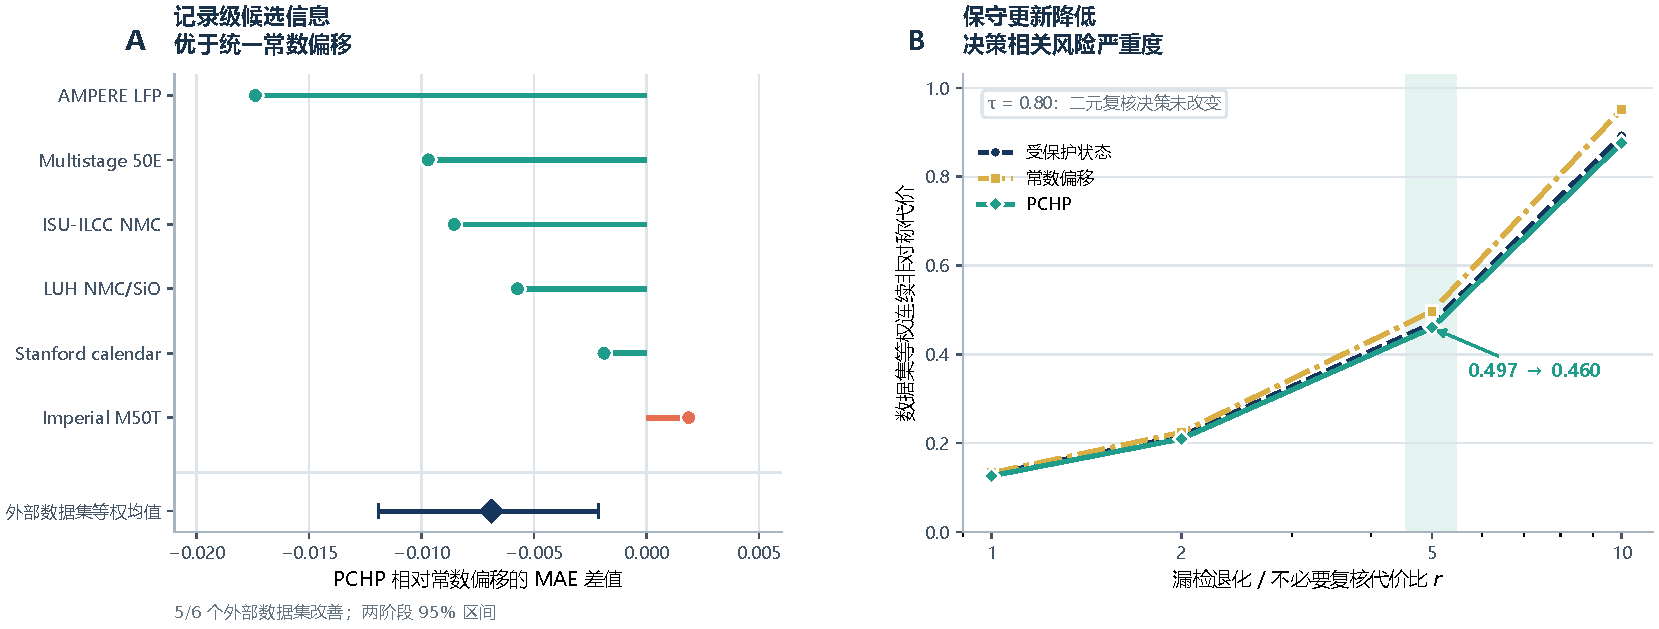
\includegraphics[width=\textwidth]{fig7_external_mechanism_decision_zh.pdf}
  \caption{协议冻结的外部机制确认与决策代价分析。\textbf{A}，六个外部电池数据集上的 PCHP 减开发集常数偏移 MAE；负值表示 PCHP 更优，菱形与区间表示数据集等权均值及两阶段数据集—电芯 bootstrap $95\%$ 区间。\textbf{B}，随漏检退化相对不必要复核代价比增加的数据集等权连续非对称代价。在主要设定 $r=5$ 下，PCHP 相对于常数偏移和受保护状态均降低代价；$\tau=0.80$ 时的二元复核决策保持不变。$9{,}712$ 条记录嵌套于 $659$ 个电芯，电芯嵌套于六个数据集。}
  \label{fig:external_mechanism_decision_zh}
\end{figure}

\subsection{强无保护比较器揭示损害控制与精度权衡}

源域调优的无保护因果比较器将域等权 MAE 从 $0.07524$ 降至 $0.05470$。它相对于受保护基线的配对差为 $-0.02054$，域 bootstrap $95\%$ 区间为 $[-0.03364,-0.00675]$，胜/平/负为 $10/0/2$。PCHP 保留了该增益的 $23.7\%$：其 MAE 比无保护比较器高 $0.01568$，区间为 $[0.00350,0.02725]$，胜/平/负为 $3/0/9$。合并 MICH 与 MICH\_EXP 后，效用保留率为 $24.9\%$，定性结论不变。

这种额外精度并未满足损害预算。无保护比较器在全部 $601{,}932$ 条评分记录中的 $524{,}165$ 条（$87.08\%$）超过了 $\delta=0.01$ 的位移预算；全部 $12$ 个域和 $586$ 个电芯都至少出现一次违规，最大位移为 $0.35680$。因此，两个记录数分别表示完整评分集合及其中的违规子集。PCHP 没有预算违规。该比较排除了“精度支配”的表述：PCHP 并不在精度上击败最强因果候选；它的贡献是在声明的最坏情况损害区域内保留可测量的候选效用。

\subsection{预设部署约束下的 BaSyTec 外部验证}

BaSyTec 评估满足全部预设判定标准。在 $47$ 个评估电芯中，$45$ 个满足冻结参照容量范围，形成 $2{,}969$ 条评分循环。电芯等权 MAE 从受保护因果基线的 $0.17496$ 降至 PCHP 的 $0.16510$。配对差为 $-0.00986$，配对电芯 bootstrap $95\%$ 区间为 $[-0.01000,-0.00959]$；全部 $45$ 个合格电芯均改善。独立重算在 $10^{-12}$ 内复现全部电芯聚合量；事后工况等权敏感性在所覆盖的 $23$ 个温度—倍率工况中均保持负值，区间为 $[-0.01000,-0.00958]$。PCHP 的最大位移和最大观察绝对损失遗憾在浮点容差内均为 $0.01$，最大电芯级 MAE 差为 $-0.00465$。

$0\,^{\circ}\mathrm{C}$、$1.5C$ 工况下的两个电芯均被预先设定的 $0.08\,\mathrm{Ah}$ 参照下限排除：F0009 与 F0048 的前五循环中位容量分别为 $0.06862$ 和 $0.06935\,\mathrm{Ah}$。明确标注为事后的全样本敏感性在 $47$ 个电芯和 $24$ 个工况上仍保持结论：配对差为 $-0.00986$，区间为 $[-0.01000,-0.00961]$，$47/47$ 个电芯改善。该敏感性表明排除规则没有制造效应，但不能替代冻结的 $45$ 电芯估计量。

同一确认也说明经验主张为何必须收窄。源域调优无保护比较器的 MAE 为 $0.06172$，但最大位移达到 $0.28508$，并在全部合格电芯和全部 $2{,}969$ 条记录上违反预算；PCHP 仅保留其精度增益的 $8.7\%$。此外，受保护基线对每条评分记录都低估，PCHP 在 $99.1\%$ 的记录上达到向上 $0.01$ 的预算边界；事后固定上移 $0.01$ 的 MAE 为 $0.16496$，比 PCHP 低 $0.00014$。因此，图~\ref{fig:basytec_zh} 验证了冻结的损害—效用约束并量化其精度权衡；该外部数据域本身不能区分自适应 PCHP 与简单的预算可行偏差修正。

\begin{figure}[t]
  \centering
  
\includegraphics[width=\textwidth]{fig6_basytec_confirmation_zh.pdf}
  \caption{结果盲、协议锁定的 BaSyTec 外部验证与损害控制—精度权衡。\textbf{A}，全部 $45$ 个合格电芯的 PCHP 减基线配对 MAE，负值表示 PCHP 更优；菱形和区间为电芯等权均值及对物理电芯执行 $100{,}000$ 次配对重采样所得的 $95\%$ bootstrap 区间。\textbf{B}，电芯等权 MAE 与相对受保护基线的最大逐点位移。PCHP 位于声明的 $\delta=0.01$ 区域内；固定上移 $0.01$ 是事后诊断，而源域调优无保护比较器具有前缀因果性但违反全部合格电芯的预算。循环嵌套于电芯。}
  \label{fig:basytec_zh}
\end{figure}

\begin{table}[H]
\centering
\caption{关键配对效应。差值定义为比较方法 MAE 减参照方法 MAE；区间对所述独立单位重采样，而非对单条记录重采样。无保护一行用于展示精度上限，但不满足损害预算。}
\label{tab:primary_zh}
\small
\begin{tabularx}{\textwidth}{>{\raggedright\arraybackslash}Xrrrrl}
\toprule
证据层级与比较 & 独立单位数 & 参照 MAE & 比较方法 MAE & 配对差 & $95\%$ 区间 \\
\midrule
嵌套开发主效应 & 12 个域 & 0.07524 & 0.07038 & $-0.00486$ & $[-0.00671,-0.00301]$ \\
PCHP 对匹配常数偏移对照 & 12 个域 & 0.07515 & 0.07038 & $-0.00477$ & $[-0.00808,-0.00159]$ \\
冻结外部机制：PCHP 对常数偏移 & 6 个数据集 & 0.13326 & 0.12636 & $-0.00690$ & $[-0.01192,-0.00212]$ \\
冻结外部机制：PCHP 对受保护状态 & 6 个数据集 & 0.13061 & 0.12636 & $-0.00424$ & $[-0.00745,-0.00079]$ \\
无保护候选对受保护基线 & 12 个域 & 0.07524 & 0.05470 & $-0.02054$ & $[-0.03364,-0.00675]$ \\
BaSyTec PCHP 对基线 & 45 个电芯 & 0.17496 & 0.16510 & $-0.00986$ & $[-0.01000,-0.00959]$ \\
\bottomrule
\end{tabularx}
\end{table}

\section{讨论}

\subsection{方法改变了什么能力}

PCHP 改变的是跨域电池预测的运行规则。学习模型仍负责提出有用更新，但不再单方面决定已经发布的健康记录。受保护因果状态明确了需要保护的预测，推论~\ref{cor:viability_kernel_zh} 则把递归可行区间刻画为在任意未来非增受保护状态路径下仍可继续执行的全部当前输出。推论~\ref{cor:optimality_zh} 进一步表明，最终输出不是该核内的任意一点，而是在完整声明约束下对当前学习候选保持最大保真度的唯一更新。定理~\ref{thm:nonexpansive_zh} 进一步保证：当输出约束固定时，完整递归级联不会放大任一冻结预测器中的有界差异。最终保证既不依赖未知结果，又可以在线执行。它不同于回顾性平滑：后者即使不读取标签，仍可能违反未来信息边界；它也不同于无约束目标适应：后者在未知数据域中的增益可能转为负值。

次级骨干分析为这一结构性主张补充了经验边界：同一组冻结输出约束在一个线性模型族和两个提升树模型族上，无须针对骨干重新调参仍保持效用。该结果排除的是所评估模型族内的 ExtraTrees 特异性，而不是对所有可能候选架构均完全无依赖。

定理~\ref{thm:harm_region_zh} 还排除了对“安全更新”的误读：在不对隐藏真实值作任何假设时，任何方法只要移动点预测，就不可能相对于基线对所有可能真实值都保持不劣。因此，正预算并不是为了证明方便而引入的松弛，而是允许任何非平凡结果未知更新所必须支付的代价。PCHP 将这一代价显式化，并且只在精确损害域与在线轨迹约束的交集中使用它。

匹配控制表明，PCHP 不只是保守裁剪。在开发域中，预算可行偏移与同化率均匹配后，相对于投运初期参照的记录级信息仍具有额外效用，而且优势贯穿全部正预算网格。六个外部数据集上的协议冻结实验进一步复现了这种区分：PCHP 在五个数据集上获胜，并使数据集等权误差相对于开发集精确选出的常数偏移降低 $5.18\%$。这构成对算法运行机制的直接外部证据：自适应候选信息能够在固定输出约束内贡献价值。本文检验的是这一算法运行机制，而不是微观电化学反应路径。

\subsection{面向电池运行的信息含义}

投影理论可以迁移至其他领域，但本文约束来自一个具体的电池决策问题。在换电站、车队场站或质保监测中，部分充电测量随日常运行到达，而参考容量需要专门安排的表征测试 \citep{liu2023rapid,zhang2024flexible}。当供应商、化学体系或运行协议发生变化时，源模型标定最可能失效，运营方却仍须决定继续运行还是发起诊断。PCHP 利用相对于投运初期参照的充电响应变化即时调整估计，限制未经验证更新可能增加的预测误差，并禁止未来测量改写既有决策历史。外部决策代价分析量化了这一价值：当漏检退化与不必要复核的代价比为 $5{:}1$ 时，决策相关误差严重度相对于匹配常数偏移下降 $7.54\%$，同时以 $80\%$ 容量保持率为阈值的二元复核决策保持不变。长期容量衰减为非增趋势提供工程动机；为识别短时恢复或测量回弹，原始观测仍应保留。

\subsection{BaSyTec 评估与损害控制—精度权衡}

BaSyTec 实验检验的是：在新的实验室、电芯类型和 $24$ 工况应力网格上，容量访问之前冻结的预测产物能否在保持全部声明损害检查的同时改善受保护基线。该检验通过；事后全工况敏感性进一步表明，预设的低参照排除没有制造效应方向。由于评分电芯位于预先声明的模型支持范围内，该结果支持既定目标约定下的相对效用；但它不能把工况特定的老化循环容量转化为标准化 RPT SOH，也不能建立测试协议之外的电化学有效性。

BaSyTec 呈现近乎一致的基线低估，因此固定正向偏移的精度略高。该结果仍然重要：它证明冻结的部署约束能够迁移到新的实验室项目，并量化执行损害预算所放弃的精度。六数据集确认则回答 BaSyTec 单独无法回答的互补问题：在误差方向异质的外部数据集上，PCHP 在通过全部确定性检查的同时优于开发集常数偏移。两项实验由此分别验证约束迁移与自适应机制价值，无须要求单一数据集同时证明两者。

\subsection{损害预算的选择}

预算 $\delta$ 以归一化容量单位表示，控制一个清晰的工程权衡：较小预算更紧密地保护既有记录，较大预算则允许更多自适应收益。冻结的 $\delta=0.01$ 将每次外部更新限制在一个归一化容量百分点内；在六数据集审计中，这一保守工作点降低了连续决策代价，同时没有改变以 $80\%$ 容量保持率为阈值的二元复核决策。不同车队可以依据维护和质保后果选择不同工作点。补充材料的理论附录给出了不等后果对应的精确方向半径，以及与已发布前缀相容的最小时变预算。

工程标定应首先冻结受保护决策、资产时间范围和成本边界，例如维护时点、可避免停机、质保责任，或另有工程依据的安全相关后果。对于预测 $p$ 和随后测得的容量保持率 $y$，可采用局部方向代价近似
\begin{equation}
  \ell_{\mathrm{eng}}(p,y)
  =c_{\mathrm{under}}(y-p)_{+}
  +c_{\mathrm{over}}(p-y)_{+},
  \label{eq:engineering_cost_zh}
\end{equation}
其中，$p<y$ 表示低估容量保持率，可能导致过早干预；$p>y$ 表示高估容量保持率，可能导致延迟干预。应当依据运营方历史记录，或通过预先登记的工程专家赋值，在声明的小扰动 $\Delta y>0$ 上估计
\begin{equation}
  c_{\mathrm{under}}=\frac{\Delta C_{\mathrm{early}}}{\Delta y},
  \qquad
  c_{\mathrm{over}}=\frac{\Delta C_{\mathrm{late}}}{\Delta y}.
  \label{eq:engineering_weights_zh}
\end{equation}
标定时应将正、负两个扰动输入同一维护或质保规则；若化学体系、任务工况或电芯年龄显著改变代价，则分层估计权重，并在访问目标结果之前冻结点估计或保守分位数。给定决策损失预算 $\eta$，独立允许区间为
\begin{equation}
  \left[b-\frac{\eta}{c_{\mathrm{under}}},
        b+\frac{\eta}{c_{\mathrm{over}}}\right].
  \label{eq:engineering_interval_zh}
\end{equation}
本文以标准化权重构造可复现的后果比例，并在 $r=5$ 时观察到 $7.54\%$ 的代价下降。实际部署可依据运营台账，将其替换为货币、停机、质保或经过验证的安全代价。若真实规则具有强非线性，则应以相应决策损失替换式~\eqref{eq:engineering_cost_zh}，并重新推导其精确可行集。

\subsection{统计解释}

确定性证书逐记录成立，不需要抽样假设；经验效用的不确定性则遵循数据层级。开发阶段由 $12$ 个完整数据域支撑，$601{,}932$ 条记录是重复观测而非独立迁移。外部机制确认以六个数据集为顶层迁移单位、以 $659$ 个电芯为嵌套重复，因此 bootstrap 先重采样数据集，再重采样电芯。BaSyTec 以 $45$ 个电芯支撑冻结项目内效应。各区间据此在与主张相符的层级刻画异质性，避免通过合并记录夸大证据量。

有限样本敏感性表明，负向域等权均值并非只由百分位 bootstrap 的计算方式产生。开发主效应和积分预算路径的精确符号翻转值分别为 $0.00098$ 与 $0.00781$，Student-$t$ 的 $95\%$ 区间分别为 $[-0.00703,-0.00269]$ 与 $[-0.01172,-0.00217]$。PCHP 相对于匹配常数偏移对照的对应结果为 $0.01660$ 与 $[-0.00858,-0.00097]$；但由于 PCHP 只在 $9/12$ 个域获胜，其仅使用方向的精确符号检验值为 $0.145996$。因此，现有证据支持的是存在域间异质性的“域等权平均效用贡献”，而不是普适支配，也不是“随机抽取一个新域时改善概率大于一半”的主张。以上数值均为基于已打开开发域的描述性事后敏感性结果。

确认强度取决于评价证据是否影响被检验的设计。BaSyTec 的预测在容量访问前冻结，因而属于结果盲确认。六数据集实验采用另一种同样有效的边界：数据档案虽曾在无关分支中出现，但其结果或汇总均未改变 PCHP、比较器、估计量、代价协议或判定标准，因此构成未受这些数据影响的协议冻结外部机制确认。两种设计提供互补证据；未来独立实验室复现可进一步扩展可迁移范围。

\section{局限性与失效模式}

该保证相对于指定受保护因果状态成立。PCHP 控制的是更新的增量损害，不能修复有偏基线、不兼容容量标签、分布偏移或不安全电池；非扩张性控制算法扰动传播，而不是校准误差或物理风险。度量损失定理与有界平方损失构造均依赖各自声明的结果空间，新的非连续决策损失需要重新推导可行集。

严格非增是一种运行趋势表征，可能抑制真实短时容量恢复或测量回弹，因此应同时保存原始观测与投影趋势。当前方法还假设前五次充电记录能够构成有效投运参照；若电芯在进入监测前已发生未观测老化，或初始记录被污染，该假设可能失效。PCHP 目前始终返回有界估计，未来可增加可估计性检查或拒绝输出机制。

实证覆盖广泛，但仍基于公开数据。十二域分析属于回顾性开发证据；六个外部数据集曾在无关分支中被打开，尽管其结果没有影响冻结方法与评价协议。BaSyTec 属于结果盲确认，但仅代表一个实验室项目，其冻结支持规则排除了两个低参照电芯。补充材料中的 NASA 分析仅作为绝对目标不兼容的单项目压力测试，不作为绝对容量保持率估计的效用证据 \citep{saha2007nasa}。下一步应在更多化学体系与任务工况中开展前瞻车队重放和独立实验室复现。最后，标准化决策代价比证明了运维相关性，但不能替代具体场站对货币、停机、质保和安全代价的标定。

\section{结论}

PCHP 使跨域电池容量保持率的学习式更新能够在容量结果到达之前按照明确约束执行。该方法把受保护预测转换为前缀因果状态，并使利用投运初期变化的候选只能通过精确递归可行的损害预算区间，从而获得前缀不变性、非增输出、每条记录 $O(1)$ 的在线执行、紧的逐记录绝对损失界，以及前缀 $\ell_\infty$ 非扩张性。十二域嵌套评估在全部更新满足 $0.01$ 预算的同时，使域等权 MAE 下降 $0.00486$。六个外部数据集上的协议冻结确认进一步表明，在 $659$ 个电芯上，自适应候选相对于开发数据精确选出的常数预算可行偏移改善 $0.00690$，两阶段 $95\%$ 区间完全低于零。当漏检退化代价为不必要复核的五倍时，连续决策风险下降 $7.54\%$，且以 $80\%$ 容量保持率为阈值的二元复核决策保持不变。BaSyTec 验证了新实验项目中的部署约束迁移，无保护比较器则量化了执行损害预算造成的精度权衡。上述结果确立了 PCHP 作为自适应锂离子电池容量保持率估计风险控制层的理论严谨性与实际价值。

\section*{稿件准备过程中生成式人工智能与人工智能辅助技术的使用声明}

在本研究准备过程中，第一作者使用 OpenAI Codex 辅助研究代码开发与核验、文献检索组织、稿件结构设计、翻译和语言编辑。第一作者对全部来源主张、数学推导、分析、代码输出、图表和正文进行了人工审查与独立核验；两位作者对最终稿件承担责任。所有科学图表均由所报告的数据和脚本以程序化方式生成；稿件图表未使用生成式图像模型创建或修改。

\section*{作者贡献声明}

吴雨阳：概念构建、方法设计、软件实现、验证、形式分析、研究实施、数据整理、可视化、初稿撰写及审阅修改。姜爱萍：研究监督、项目管理及稿件审阅修改。

\section*{数据可用性}

精确开发快照 BatteryLife\_Processed v11 已由 Zenodo 以 CC BY~4.0 归档 \citep{batterylife2026processed}。六数据集确认使用所引 A123/LFP、Imperial M50T、Luh NMC/C--SiO、ILCC 变使用条件、Stanford 日历老化和多阶段老化数据源 \citep{wheeler2025lfp,kirkaldy2024comprehensive,luh2024dataset,li2024varyingusage,lam2025calendar,stroebl2024multistage}。包含 $48$ 个电芯的拜罗伊特退化路径数据集由 Zenodo 以 CC BY~4.0 发布 \citep{roder2025degradationdata}。全部第三方档案仍遵循原提供方的访问、署名与再分发条款，本文不重新分发其原始压缩包。作者生成的复现发布包包含数据获取说明、源文件与工件哈希、冻结外部协议、按数据集与电芯聚合的证据、独立证书与统计重放检查，以及全部论文图生成输入和脚本，现已采用 MIT License 公开于 \href{https://github.com/xiansuqiushui-dotcom/pchp-battery-capacity-retention}{GitHub 代码仓库}。该发布包不取代任何第三方条款；完整重训与外部重放仍须按原提供方要求自行下载数据。

\section*{基金声明}

本研究未获得公共、商业或非营利部门资助机构的专项基金资助。

\section*{利益冲突声明}

作者声明不存在可能影响本文工作的已知竞争性经济利益或个人关系。

\bibliographystyle{elsarticle-num}
\begingroup
\hbadness=2000
\bibliography{references}
\endgroup

\end{document}
